% Based on 'explaining explanations' paper: interpretable and complete; interpr: understandable to humans, simple enough using voca that is meaningful to user; explanation-producing systems;

%Compute explanation of form C /\ B -> A. By find B = MUS(not A, C) so not a and C and B so a <- B and C; BnC may generate more, so apply BnC to obtain A and B and C -> A. (This is why 'B' and nr of constraints C have to be small);
%Simplicity: size of B, C and A as small as possible, 

%Need for explanations of reasoning systems
Explainable AI research aims to fulfill the need for trustworthy AI systems that can explain their reasoning in a human-understandable way. 
As these systems employ more advanced reasoning mechanisms and computation power, it becomes increasingly difficult to understand why certain decisions are made. 
Understanding the decisions is important for verifying the correctness of the system, as well as to control for biased or systematically unfair decisions.

Explainable AI is often studied in the context of (black box) machine learning systems such as neural networks, where the ability to provide insight into what part of the (potentially large) input was most important to infer the predicted label is often crucial. 
%Another domain is explainable planning, which looks among others at answering user queries regarding a computed plan and model reconciliation.\bart{Beetje kort. Kan je daar meer over zeggen? }

%Shallow related work on quickxplain, 'explanations' in search, etc.
Explanations have been investigated as part of constraint solving before. Most notably, for explaining over-constrained problems~\cite{junker2001quickxplain} to a user. In our case we are looking at satisfiable problems with a unique solution. Also at the solving level, in lazy clause generation solvers, an explanation of a constraint is an implication of low-level Boolean literals that encode the result of a propagation step~\cite{feydy2009lazy}. Also, nogoods (unsat cores) in SAT solvers can be seen as explanations of failure during search~\cite{marques2009conflict}. These are not meant to be human-interpretable but rather to propagate efficiently.


%Difference automated reasoning and human reasoning, measuring cognitive load
We here investigate the problem of explainable constraint solving. More specifically, we aim to develop an explanation-producing system that is complete and interpretable. By complete we mean that it finds a \textit{sequence} of reasoning steps that, starting from the given problem specification, leads to the unique solution of the problem\tias{added assumption of uniqueness, though not very explicit}. An explanation of one reasoning step is an implication of the form $E \wedge S \rightarrow N$, where $E$ is \textit{evidence} namely a set of previously derived facts, $S$ is a (sub)set of constraints, and $N$ is a set of newly derived facts that follow from $E$ and $S$. Measuring the interpretability of a reasoning step is difficult, but our guiding principle is that of simplicity, where smaller and simpler $E \wedge S \rightarrow N$ explanations are better. 
\bart{The above is phrased very generic. That is good. However, sequences such as the ones we consider here need no always exist, e.g., in case a logic problem does not ahve a unique solutoin...}
\tias{If it has NO solution OK, but if where does problem arise for above statement for multiple solutions? We need to make our assumputions stronger: that there is a unique solution?}
\bart{Actually, our techniques would also work for UNSAT problems. It would then generate  a human-understandable UNSAT proof}


Gilpin et al.~\cite{DBLP:conf/dsaa/GilpinBYBSK18} define interpretable explanations as ``descriptions that are simple enough for a person to understand, using a vocabulary that is meaningful to the user''. For the constraints $C$, we choose to represent them in natural language. In the case of logic grid puzzles this is an obvious choice as the constraints are \textit{clues} that are given in natural language. For the previously and newly derived facts $E$ and $N$, we choose a visual representation of those facts in the solution structure. For logic grid puzzles this is the logic grid (see Figure ...).

%HolyGrail challenge and related work
Our work is motivated by Eugene Freuder's ``Holy Grail Challenge'' which had as objective  to provide automated processing of a simple, restricted class of problems, logic grid puzzles specifically, ranging from natural language processing, to solving, and explanining \cite{}. 
An earlier version of this system was the challenge winner at the workshop. The challenge has its roots in early work of Eugene Freuder \cite{DBLP:conf/aaai/SabinF96,DBLP:conf/aaai/SqalliF96}.
There has been a lot of previous work on automatically \emph{solving} logic grid puzzles, starting from the natural language clues \cite{related,work}. 
While our system also has this capability (see Section \ref{sec:holistic}), the focus of this paper is on the novel explanation-producing part of the system.

The explanation-generating techniques we develop can be applied in a multitude of use cases. 
For instance, our tool can explain the entire sequence of reasoning, such that a user can debug either the reasoning system or the set of constraints that are given as problem specification. 
As our approach starts from an arbitrary set of facts, it can also be used as a virtual assistant when a user is stuck in solving a problem, where the system will explain the simplest possible next move, or in an interactive setting where the user interactively assigns facts himself or by the system \bart{I didnt get this last one.}. 
Finally, our measures of simplicity of reasoning steps can be used to estimate the difficulty of solving a problem for a human, and hence order problems by difficulty for training purposes.

%challenge 1: abstraction in self-contained reasoning step
%challenge 2: ordering
%challenge 3: computation efficiency
%The challenge in making an explanation-producing constraint solving method is choosing the right level of abstraction for the constraints and explanations, defining what a good ordering of the explanations is, and extracting a complete sequence of good explanations in a computationally efficient way. The search for a sequence of small explanations is much more computationally intensive than searching for a satisfying solution as it requires repeatedly solving subparts of the problem.

\tias{term 'ordering' disappears? not ordering but sequencing}

%Contributions: (eerste aanzet!!!)
Our contributions are the following:
\begin{itemize}
	\item We formalize the problem of finding a good ordering of interpretable reasoning steps
	\item We investigate different measures of interpretability and quality of ordering
	\item We propose algorithms to approximate the ???some hardness result??? problem of finding the best ordering \bart{Hardness result is not very easy to get due to quite specific form of the puzzles... } 
	\item We experimentally demonstrate the quality and feasibility of the approach in the domain of logic grid puzzles
\end{itemize}

\tias{stress step-wise explanation, need for sequence of small steps; finding these small steps is the main difficulty}
\tias{Add model-based argument: that it is not a black box mimicing, but the actual steps following from the problem representation (instead of learned representation)}

In contrast, our proposed method works for any type of constraint and any combination of constraints, and automatically infers a minimal set of facts and constraints that explain an inference step, without using any problem-specific knowledge.

\bart{Mention running example? Mention that this is a very hard puzzle (80 people at an AI conference received it; 4 solved it; many more tried)? } \tias{go ahead... somewhere small ; )}

\tias{Paper organization}

\begin{figure}[t]
\centering
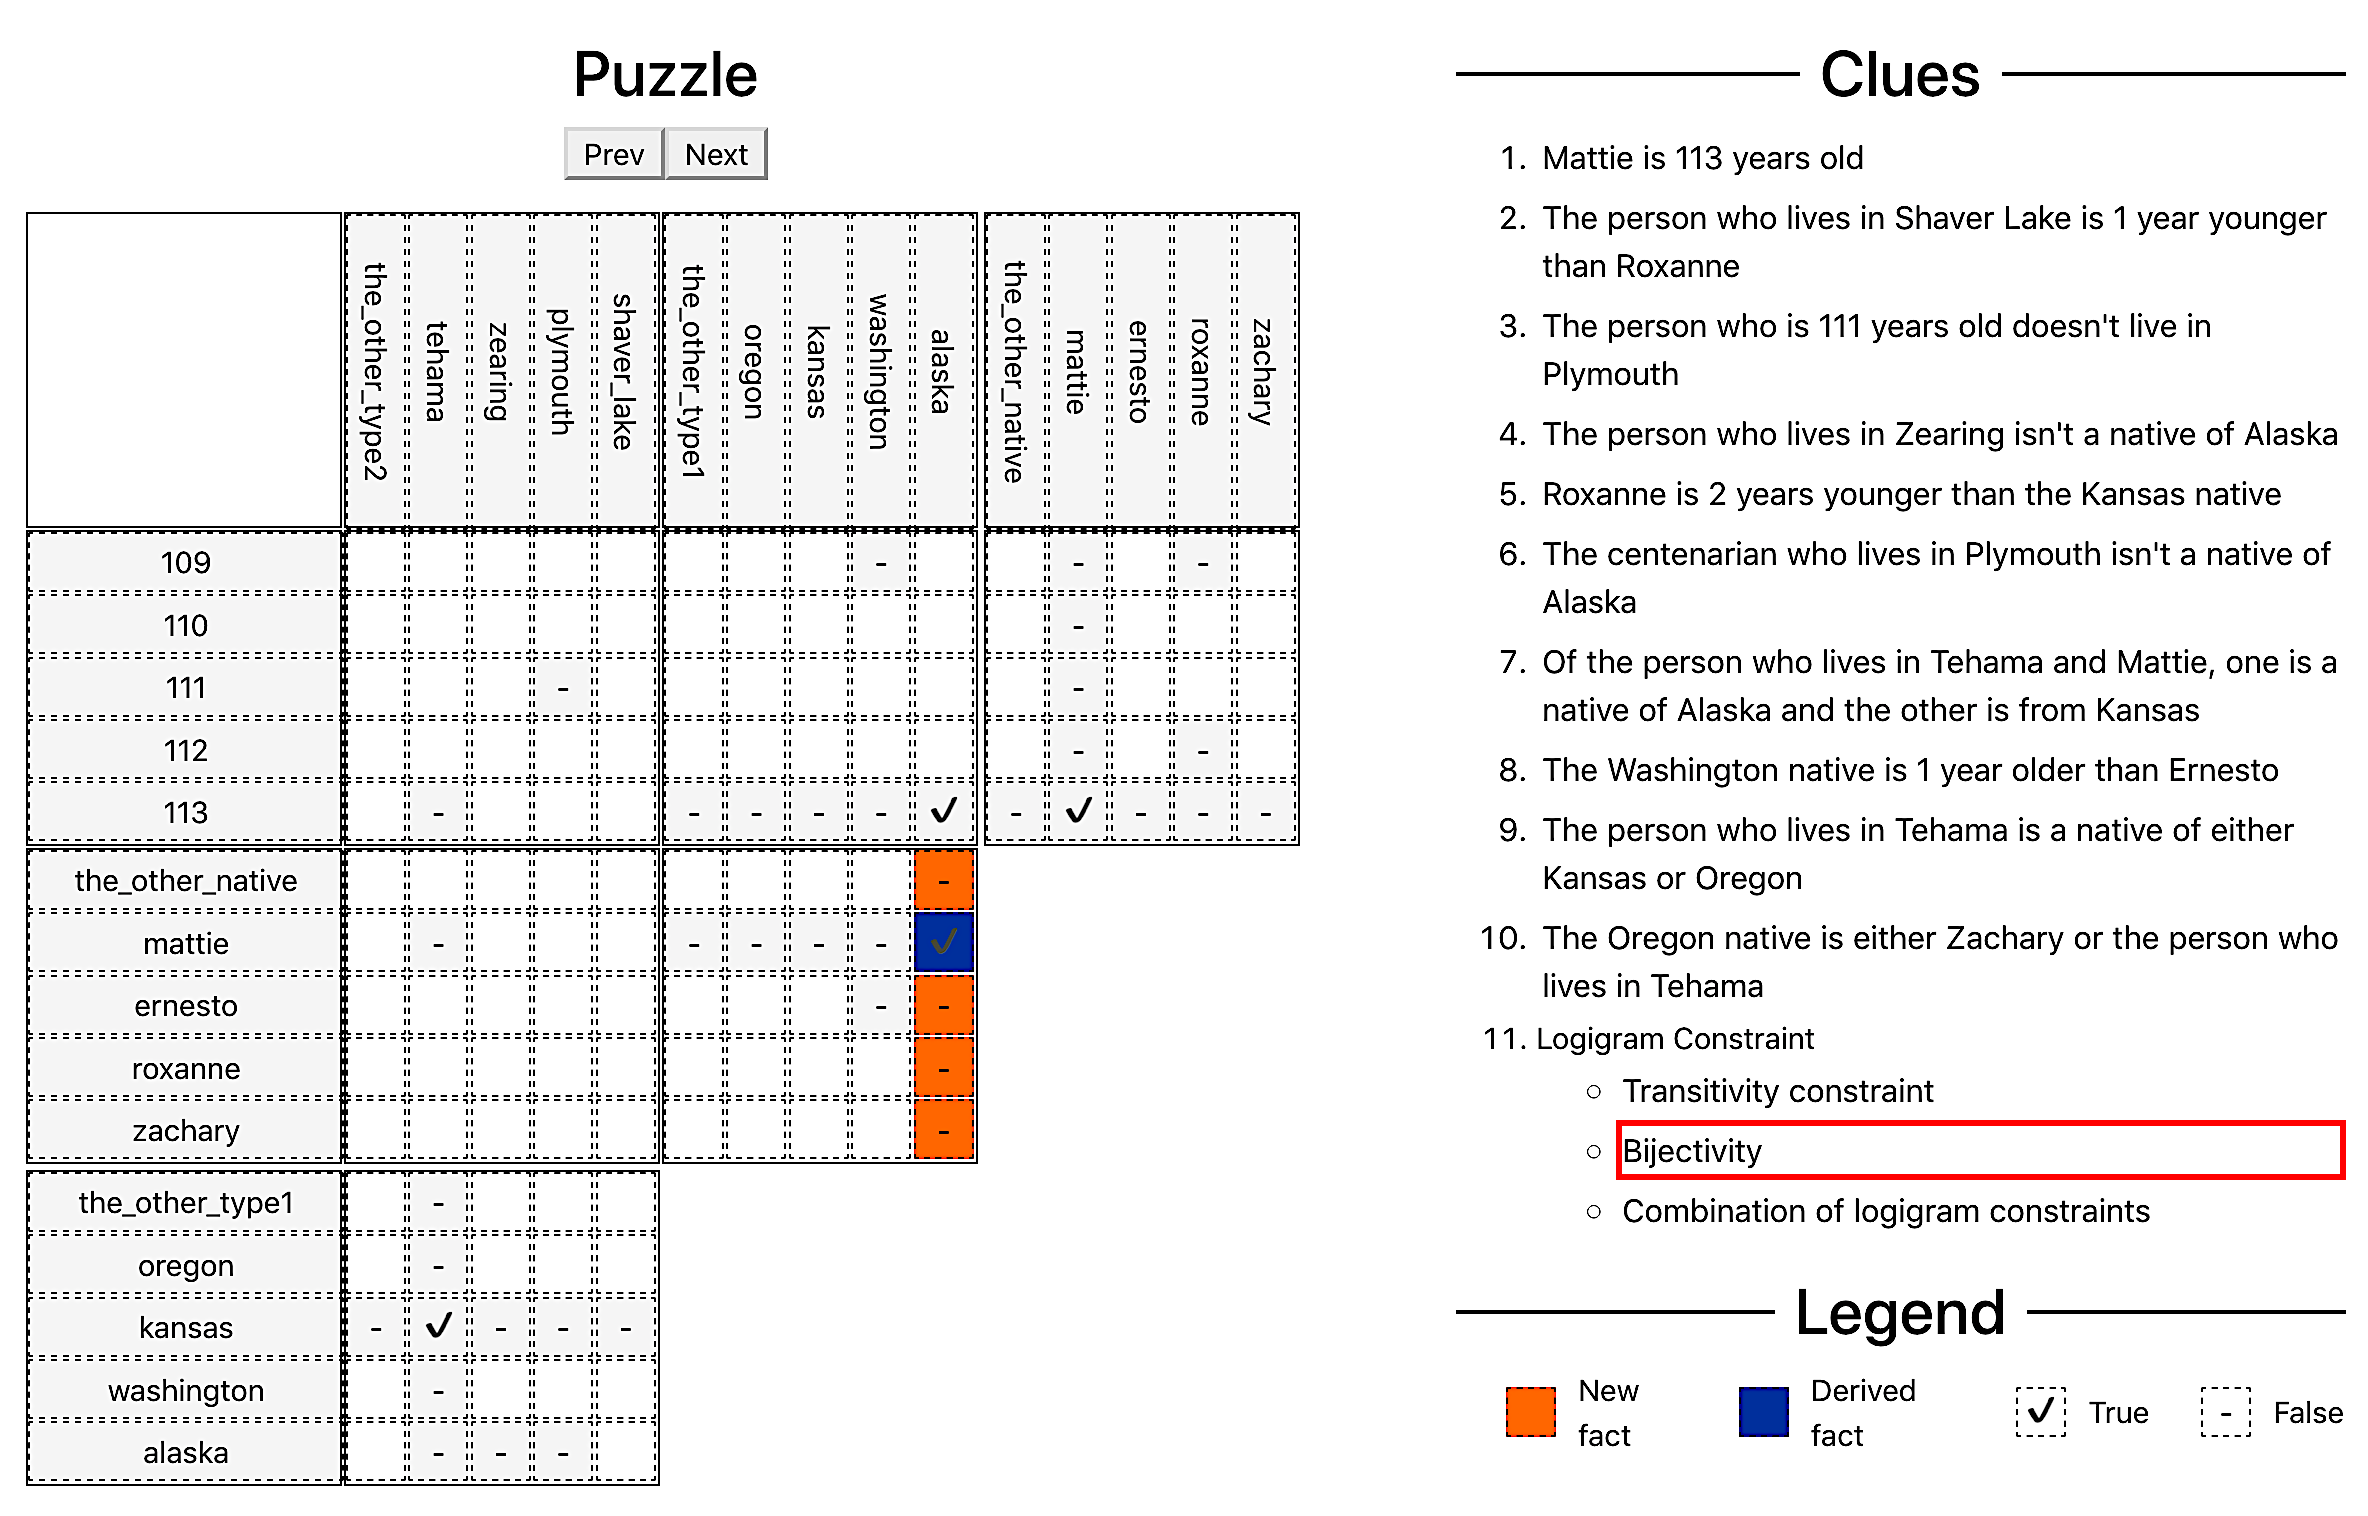
\includegraphics[width=1\linewidth]{zebra_screen}
\caption{Demonstration of explanation visualisation.}
\label{fig:zebrascreen}
\end{figure}

